% Make nice A4 pages for print:
%\usepackage{pgfpages}
%\pgfpagesuselayout{resize to}[a4paper,border shrink=5mm,landscape]

\beamertemplatenavigationsymbolsempty

\setbeamertemplate{bibliography item}[text]

\usepackage[type={CC},modifier={by-sa},version={4.0}]{doclicense}

\usepackage[utf8]{inputenc}
\usepackage{hyperref}
\usepackage{breakurl}
\usepackage{graphicx}
\usepackage{pgfplots}
\usepackage{pgf}
\usepackage{tikz}
\usetikzlibrary{positioning}
\usetikzlibrary{arrows}
\usetikzlibrary{decorations.markings}
\usetikzlibrary{calc}
\usetikzlibrary{matrix}
\usetikzlibrary{shapes}
\usetikzlibrary{decorations.pathmorphing}
\usetikzlibrary{fit}
\usetikzlibrary{backgrounds}
\usetikzlibrary{plotmarks}
\usepackage{stmaryrd}
\usepackage{listings}
\usepackage{pdflscape}
\usepackage{perpage}
\usepackage{appendixnumberbeamer}

%\usepackage[thmmarks,amsmath,amsthm]{ntheorem} % already included in beamer
\usepackage{thm-restate}

\usepackage[sort&compress,numbers]{natbib}  % to be have \citet, \citeauthor, \citeyear

\MakePerPage{footnote}

\tikzstyle{o}=[r,ppBlue]
\tikzstyle{r}=[thick,rectangle,align=center]
\tikzstyle{t}=[r,ppTrans] %,font=\bfseries]
\tikzstyle{dd}=[densely dashed]
\tikzstyle{n}=[r,ppBlue]
\tikzstyle{p}=[r,ppRed]
\tikzstyle{ppRed}  =[draw=red,  fill=  red!20]
\tikzstyle{ppBlue} =[draw=blue, fill= blue!20]
\tikzstyle{ppGreen}=[draw=green,fill=green!20]
\tikzstyle{ppTrans}=[draw=none, fill=none]

\usetheme{Warsaw}

\useoutertheme[subsection=true]{smoothbars}
%\useoutertheme[subsection=false]{miniframes}

\definecolor{bblue}{HTML}{D7DF01}	% yellow-ish actually, for better black/white printing
\definecolor{rred}{HTML}{C0504D}
\definecolor{ggreen}{HTML}{9BBB59}
\definecolor{ppurple}{HTML}{9F4C7C}
\definecolor{lightgray}{rgb}{0.3,0.3,0.3}
\definecolor{lightergray}{rgb}{0.9,0.9,0.9}
\definecolor{UniBlue}{RGB}{83,121,170}

\DeclareTextFontCommand\textintro{\normalfont\bfseries\itshape} % nice!
\newcommand{\intro}[2][]
{%
	\textintro{#2}%
}
\newcommand{\empha}[2][]
{%
	\emph{#2}%
}

%\theoremstyle{plain}
\newcounter{reqcounter}
\newtheorem{requirement}[reqcounter]{Requirement}

%setbeamercolor{structure}{fg=violet}

\makeatletter
\def\th@task{%
    \normalfont % body font
    \setbeamercolor{block title example}{bg=orange,fg=white}
    \setbeamercolor{block body example}{bg=orange!20,fg=black}
    \def\inserttheoremblockenv{exampleblock}
  }
\makeatother

\theoremstyle{task}
\newtheorem{task}{Task}

\newenvironment{assignment}%
{%\setbeamercolor{background canvas}{bg=violet}%
%\setbeamercolor{structure}{fg=cyan!90!black}%
 \setbeamercolor{frametitle}{bg=orange,fg=white}
\begin{frame}}%
{\end{frame}}%

\AtBeginSection[]{
  \begin{frame}
  \vfill
  \centering
  \begin{beamercolorbox}[sep=8pt,center,shadow=true,rounded=true]{title}
    \usebeamerfont{title}\insertsectionhead\par%
  \end{beamercolorbox}
  \tableofcontents
  \vfill
  \end{frame}
}




\pgfplotsset{compat=1.14}
\author{Markus Raab}


% TODO: Reduce more to learning outcome

\title{L01 Configuration Settings}
\date{}

\begin{document}
\section{Elektra}
\begin{frame}
	\frametitle{Elektra~\cite{raab2016elektra}}
	\begin{itemize}[<+->]
	%	\item \citet{holland2001nofutz}~defined \empha{futzing} to denote \enquote{tinkering or fiddling experimentally}
	%	\item With \intro[no-futz computing]{no-futz computing} \citet{holland2001nofutz} mean \enquote{that futzing should be allowed, but should never be required}
		\item \elektra{} is a framework implementing a modular \intro{configuration specification language} for configuration settings
		\item \intro{configuration specification languages} mitigate misconfigurations
	%	\item In \elektra{} we use properties to specify configuration settings and configuration access
		\item \elektra{} enables \intro[no-futz computing]{no-futz computing} \cite{holland2001nofutz},
			i.e., error-prone \enquote{tinkering or fiddling experimentally} \enquote{should be allowed, but should never be required}
	\end{itemize}
\end{frame}

\begin{frame}
	\frametitle{Elektra as Virtual Filesystem}
	\begin{itemize}
	\item configuration files are seen like ``block devices''
	\item are mounted with respective filesystem drivers into the filesystem
	\item many tools and APIs evolved to work with files
	\item Idea of Elektra: establish a similar ecosystem for configuration
	\end{itemize}
\end{frame}

\begin{frame}
	\frametitle{Why is Elektra not a Filesystem then?}
	\begin{itemize}
	\item API semantics: key/value get/set
	\item namespaces: based on established semantics
	\item many features essential for misconfiguration hardening:
		\begin{itemize}
		\item validation
		\item visibility
		\item defaults
		\item \dots (extensible specification)
		\end{itemize}
	\end{itemize}
\end{frame}

%%%%%%%%%%%%%%%%%%%%%%%%%%%%%%%%%%%%%%%%%% 
\section{Definitions}

\begin{frame}
	\frametitle{Learning Outcomes}
	Students will be able to
	\begin{itemize}
	\item remember definitions of configuration settings.
	\end{itemize}
\end{frame}

\begin{frame}
	\frametitle{Basic Definitions}
	The \intro[execution environment]{execution environment} is information outside the boundaries of each currently running process~\cite{corbato1971multics}.

	Controlling the execution environment is essential for configuration management~\cite{cons2002pan,huang2015confvalley}, testing~\cite{van2010automating,wang2009context}, and security~\cite{goldberg1996secure,schreuders2012towards,perkins2009automatically,liang2003isolated}.
\end{frame}

\begin{frame}
	\frametitle{Configuration Setting}
	\begin{definition}
\label{def:configuration-setting}
A \intro[configuration setting]{configuration setting},
or \intro[setting|see{configuration setting}]{setting} in short,
fulfills these properties:
\begin{enumerate}
\item
It is provided by the execution environment.
\item
It is \empha[consume]{consumed} by an application.
\item
It consists of a key, a configuration value, and potentially \empha{metadata}.
The \intro{configuration value}, or \intro[value|see{configuration value}]{value} in short, influences the application's behavior.
\item
It can be \empha[produce]{produced} by the maintainer, user, or system administrator of the software.
\end{enumerate}
\end{definition}

\end{frame}

\begin{frame}[fragile]
	\frametitle{Synonyms for Configuration Settings}
	\ExecuteMetaData[../../book/background.tex]{synonyms}
\end{frame}




%%%%%%%%%%%%%%%%%%%%%%%%%%%%%%%
\section{Metalevels}

\begin{frame}
	\frametitle{Metalevels}
	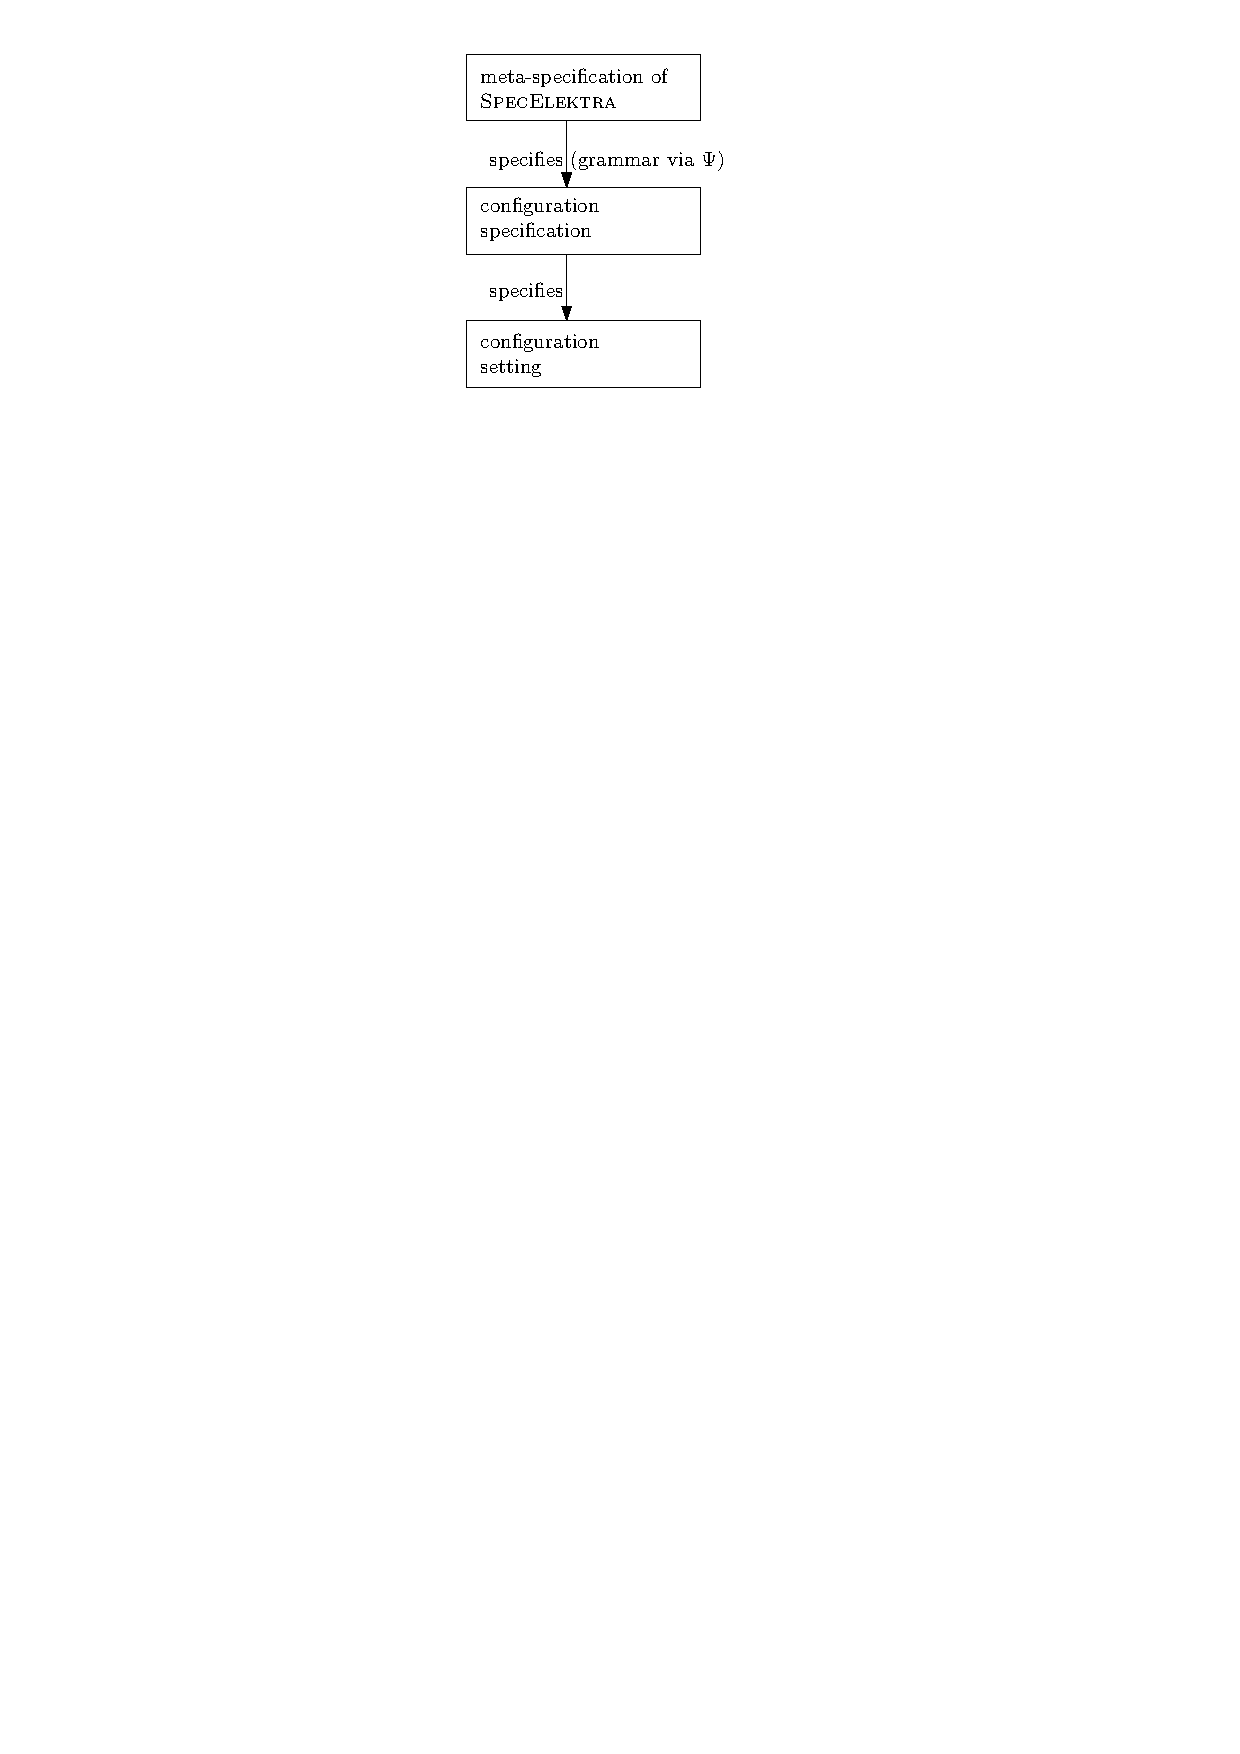
\includegraphics{metalevels}

	We will now walk through metalevels bottom-up.
\end{frame}

\begin{frame}[fragile]
	\frametitle{Configuration Settings}

	A configuration file may look like (properties format):

	\begin{code}[language=CfgElektra]
	slapd/threads/listener=4
	\end{code}

	\vspace{1cm}

	We apply these configuration settings imperatively using:

	\begin{code}[language=bash]
	kdb set /slapd/threads/listener 4
	\end{code}
\end{frame}

\begin{frame}[fragile]
	\frametitle{Specifications}
	For specifications such as:

	\begin{code}
	[slapd/threads/listener]
	  check/range:=1,2,4,8,16
	  default:=1
	  visibility:=advanced
	  description:=One thread is adequate\
		       for up to 16 CPU cores.
	\end{code}

	\vspace{0.6cm}

	We apply the specifications imperatively using:

	\begin{code}[language=bash,morekeywords={meta-set}]
	kdb meta-set /slapd/threads/listener\
		check/range 1,2,4,8,16
	kdb meta-set /slapd/threads/listener\
		default 1
	\end{code}
\end{frame}

\begin{frame}[fragile]
	\frametitle{Meta-Specifications}
	For meta-specifications such as:

	\small
	\begin{code}
	[visibility]
	type:=enum critical important user\
	      advanced developer debug disabled
	description:=Who should see this\
	     configuration setting?
	\end{code}

	\vspace{1cm}

	We apply the meta-specifications imperatively using:

	\begin{code}[language=bash,morekeywords={meta-set}]
	kdb meta-set /elektra/meta/\
		visibility type enum ...
	kdb meta-set /elektra/meta/\
		visibility description "Who ...
	\end{code}
\end{frame}

%%%%%%%%%%%%%%%%%%%%%%%%%%%%%%%
\section{KeySet}

\begin{frame}
	\frametitle{KeySet}

	The common data structure between plugins and applications:
	\vspace{1cm}

	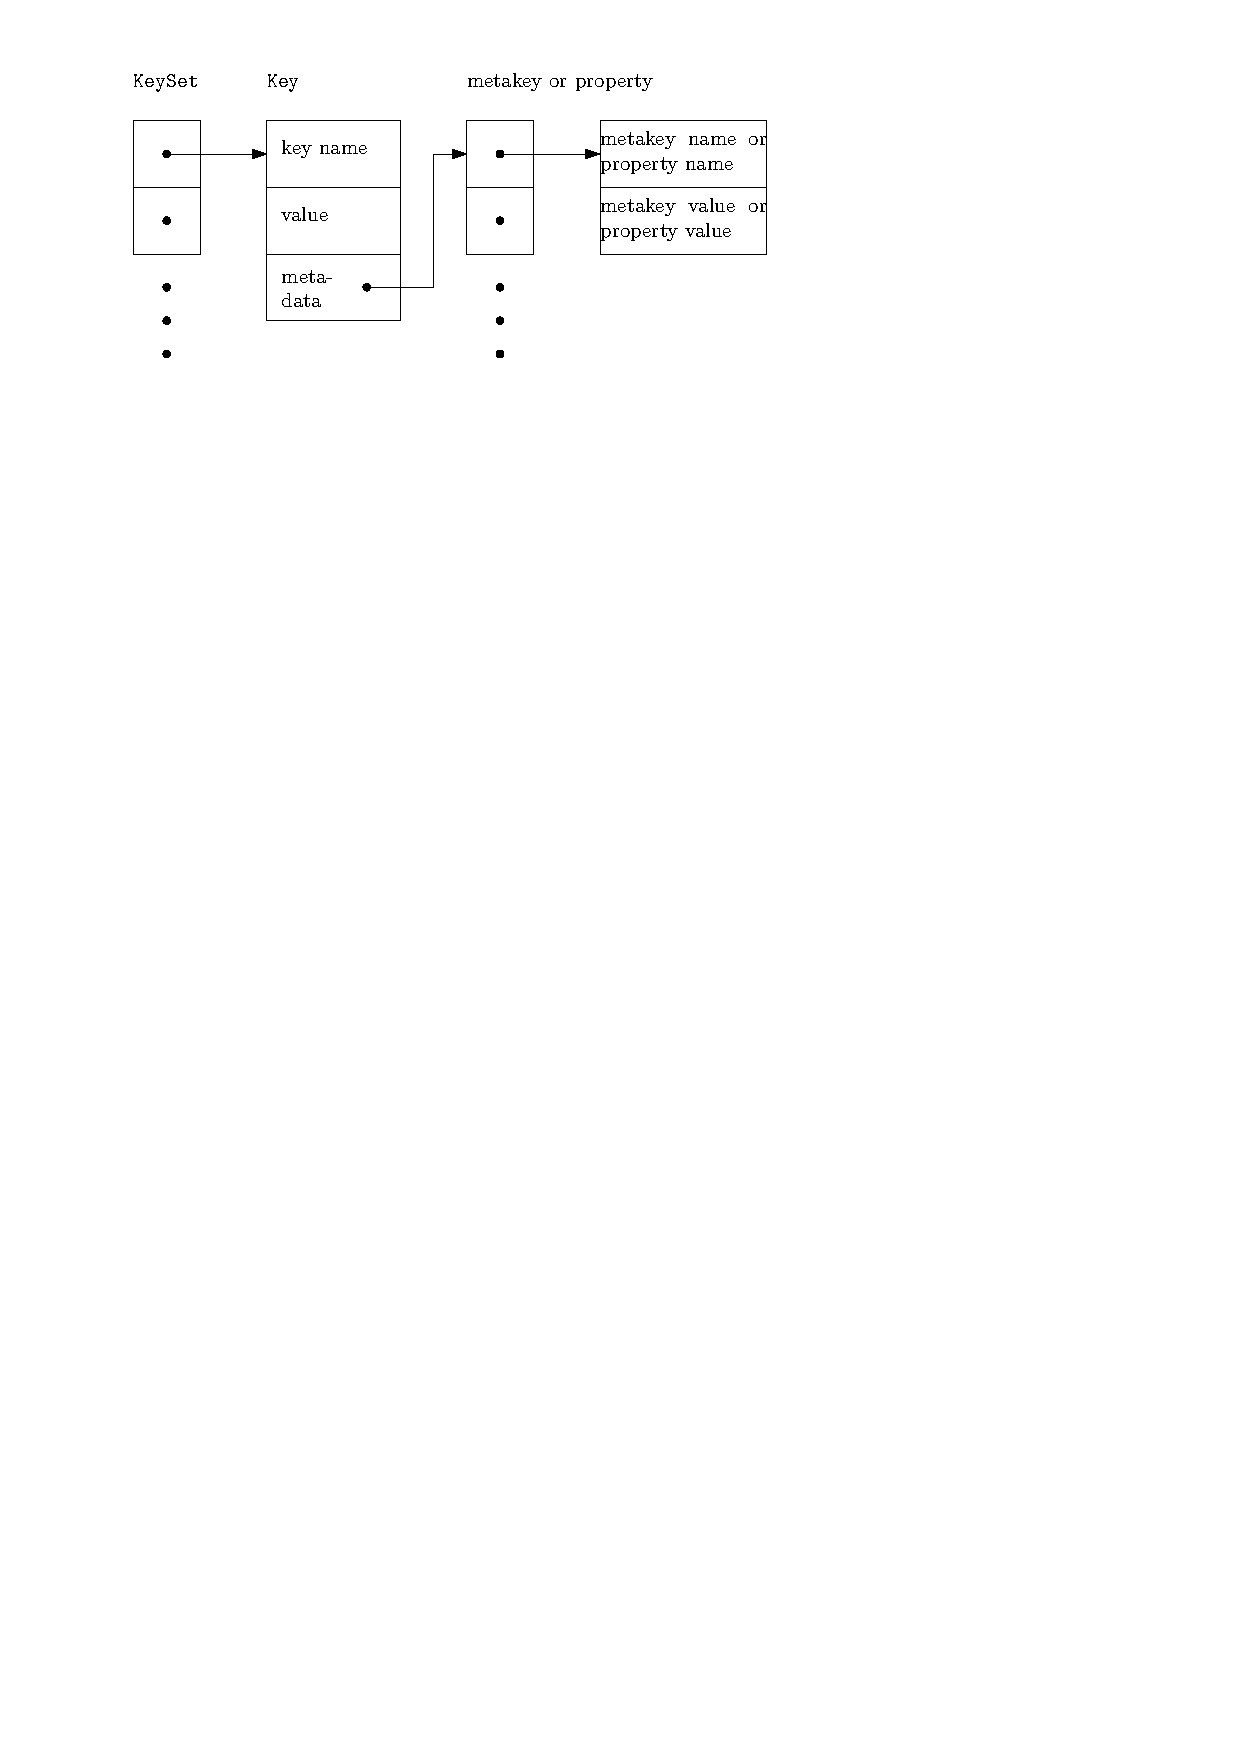
\includegraphics{keyset}
\end{frame}

\begin{frame}[fragile]
	\frametitle{Grammar}
	\begin{alertblock}{Idea}
	Use configuration file format grammar to describe both configurations and (meta-)specifications
	\end{alertblock}

	\begin{grammar}
	<KeySet> ::= \lq ksNew'\WhiteSpace(' \{ <Key> \lq , \LineBreak'  \}  \{ \lq\WhiteSpace' \} \lq KS\_END);'

	<Key> ::= \lq keyNew \WhiteSpace ('' ' <key name> \lq ''  , \LineBreak' [ <Value> ] <properties> \lq KEY_END)'

	<Value> ::=  \{ \lq\WhiteSpace' \} \lq KEY\_VALUE, \WhiteSpace '' ' <configuration value> \lq ''  , \LineBreak'

	<properties> ::= \{ \{ \lq\WhiteSpace' \} <property> \lq , \LineBreak' \}

	<property> ::=  \lq KEY\_META, \WhiteSpace " ' <property name> \lq "  , \WhiteSpace " ' <property value> \lq " '
	\end{grammar}
\end{frame}

\begin{frame}[fragile]
	\frametitle{Example}
	\begin{example}
	Given the key ^/slapd/threads/listener^, with the configuration value ^4^ and the property $\property{default} \mapsto 1$, \elektra{} emits:

	\begin{code}[gobble=4,language=Cpp]
	ksNew (keyNew ("/slapd/threads/listener",
		       KEY_VALUE, "4",
		       KEY_META, "default", "1",
		       KEY_END),
	       KS_END);
	\end{code}
	\vspace{-1em}
	\end{example}

	\pause
	\begin{alertblock}{Finding}
	We have source code representing the settings.
	If we instantiate it, we get a data structure representing the settings.
	Plugins emitting such ``configuration files'' are code generators.
	\end{alertblock}
\end{frame}

\begin{frame}[fragile]
	\frametitle{Usage in Applications}

	With the specification:
	\par
	\begin{code}[gobble=4]
	[slapd/threads/listener]
	  check/range:=1,2,4,8,16
	  default:=1
	  visibility:=advanced
	  restrict/write:=1
	\end{code}
	\par
	\elektra{Gen} gives the user read-only access to the object ^env.slapd.threads.listener^:
	\par
	\begin{code}[language=Cpp]
	std::cout << env.slapd.threads.listener;
	env.slapd.threads.listener = 3; // error
	\end{code}
	\par
\end{frame}

\begin{frame}
	\frametitle{Implementation}
	\begin{columns}[c]
	\begin{column}{6cm}
	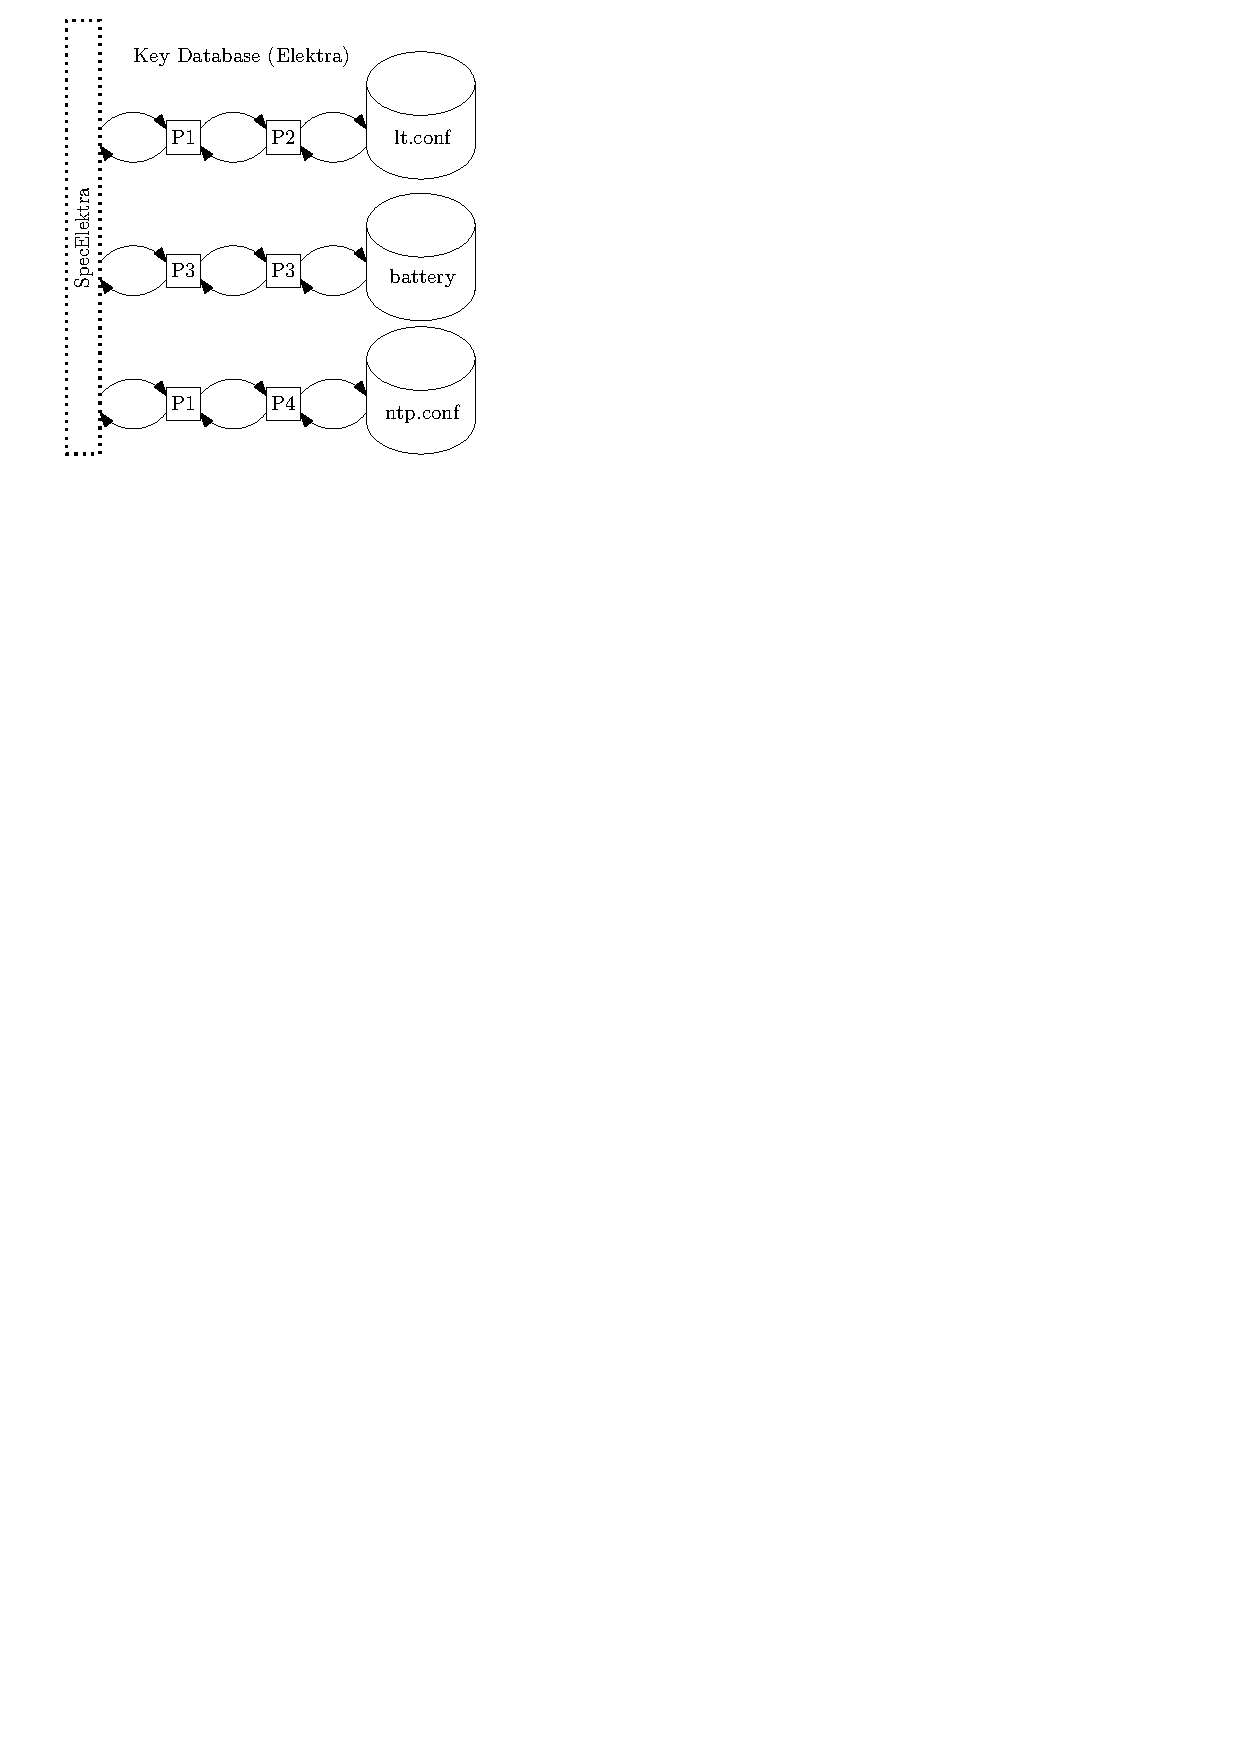
\includegraphics[scale=0.8]{horizontalmodularity}
	\end{column}
	\begin{column}{5cm}
	Cylinders are configuration files, P? are plugins~\cite{raab2016improving}.

	\begin{itemize}
	\item syntax is defined via plugins reading/writing configuration files
	\item semantics are defined via
		\begin{itemize}
		\item plugins interpreting properties
		\item generated code used by applications
		\end{itemize}
	\end{itemize}
	\end{column}
	\end{columns}
\end{frame}

%%%%%%%%%%%%%%%%%%%%%%%%%%%%%%%%%%%%%%%%%% 
\begin{frame}[fragile]
	\begin{description}[align=left]
	\item[kdb.open():]
	The first step is to bootstrap into a situation where the necessary plugins can be loaded.
	\item[kdb.get(\texttt{KeySet}):] \index{kdb.get}
	The application (initially) fetches and (later) updates its configuration settings as a key set of type ^KeySet^ from the execution environment by one or many calls to ^kdb.get^.
	%If all relevant configuration files are unmodified since the last invocation, ^kdb.get^ will do nothing.
	\item[kdb.set(\texttt{KeySet}):] \index{kdb.set}
	When a user finishes editing configuration settings, ^kdb.set^ is in charge of writing all changes back to the key database.
	%This function atomically persists a whole key set in involved parts of the execution environment.
	%In the case of an error no action takes place.
	\item[kdb.close():] \index{kdb.close}
	The last step is to close the connection to the key database.
	\end{description}
\end{frame}

\section{Meeting}
%\subsection{Recapitulation}
%{
%\shadowcolor{black}
%\shadowoffset{0.5pt}
%\usebackgroundtemplate{\includegraphics[width=\paperwidth]{pics/clouds.jpg}}%
%\begin{frame}
%	\frametitle{\shadowtext{Misconfiguration (Recapitulation)}}
%
%	\pause
%
%	\begin{itemize}
%		\item   \textcolor{white}{\shadowtext{\empha[misconfiguration]{misconfigurations}~\cite{yin2011empirical,su2007autobash,attariyan2010automating,xu2015systems} are a major cause}}\\
%			\textcolor{white}{\shadowtext{of system failures~\cite{wool2004quantitative,oppenheimer2003internet,pertet2005causes}}}
%		\item   \textcolor{white}{\shadowtext{much time is needed to fix misconfigurations~\cite{rabkin2011static,oppenheimer2003internet,yin2011empirical,mahajan2002bgp}}}
%	\end{itemize}
%\end{frame}
%}
%
%\begin{frame}
%	\frametitle{Configuration Setting (Recapitulation)}
%
%	\pause
%
%	\begin{definition}
\label{def:configuration-setting}
A \intro[configuration setting]{configuration setting},
or \intro[setting|see{configuration setting}]{setting} in short,
fulfills these properties:
\begin{enumerate}
\item
It is provided by the execution environment.
\item
It is \empha[consume]{consumed} by an application.
\item
It consists of a key, a configuration value, and potentially \empha{metadata}.
The \intro{configuration value}, or \intro[value|see{configuration value}]{value} in short, influences the application's behavior.
\item
It can be \empha[produce]{produced} by the maintainer, user, or system administrator of the software.
\end{enumerate}
\end{definition}

%\end{frame}
%
%\begin{frame}
%	\frametitle{Metalevels (Recapitulation)}
%	\begin{alertblock}{Question}
%	Describe the three Metalevels in Elektra.
%	\end{alertblock}
%
%	\pause
%	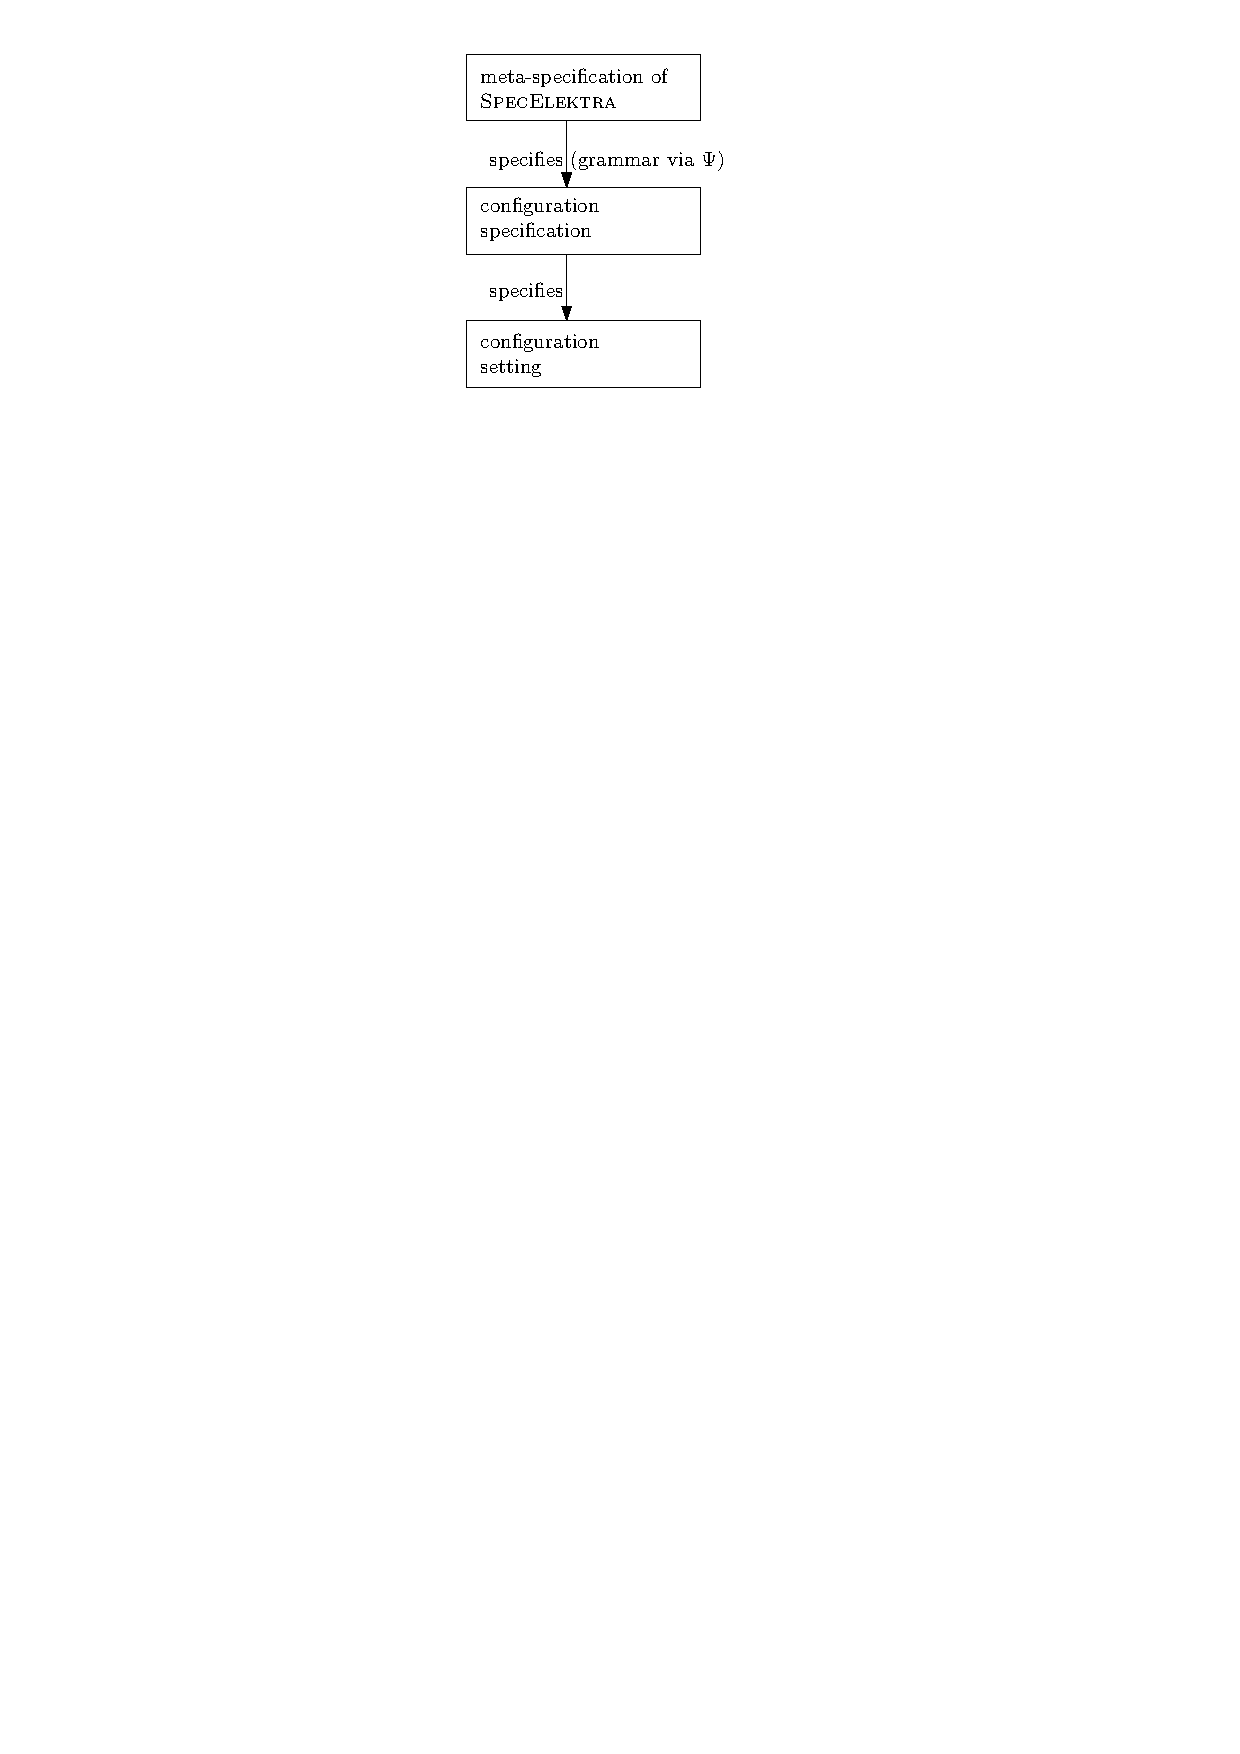
\includegraphics{metalevels}
%\end{frame}
%
%\begin{assignment}
%	\begin{task}
%	Break.
%	\end{task}
%\end{assignment}
%
%
%\begin{assignment}
%	\begin{task}
%	Is meta-data separated from or included in the data structure KeySet?
%	\end{task}
%\end{assignment}
%
%
%\begin{frame}
%	\frametitle{KeySet (Recapitulation)}
%
%	\begin{alertblock}{Question}
%	Describe the common data structure in Elektra.
%	\end{alertblock}
%
%	\vspace{1cm}
%	\pause
%
%	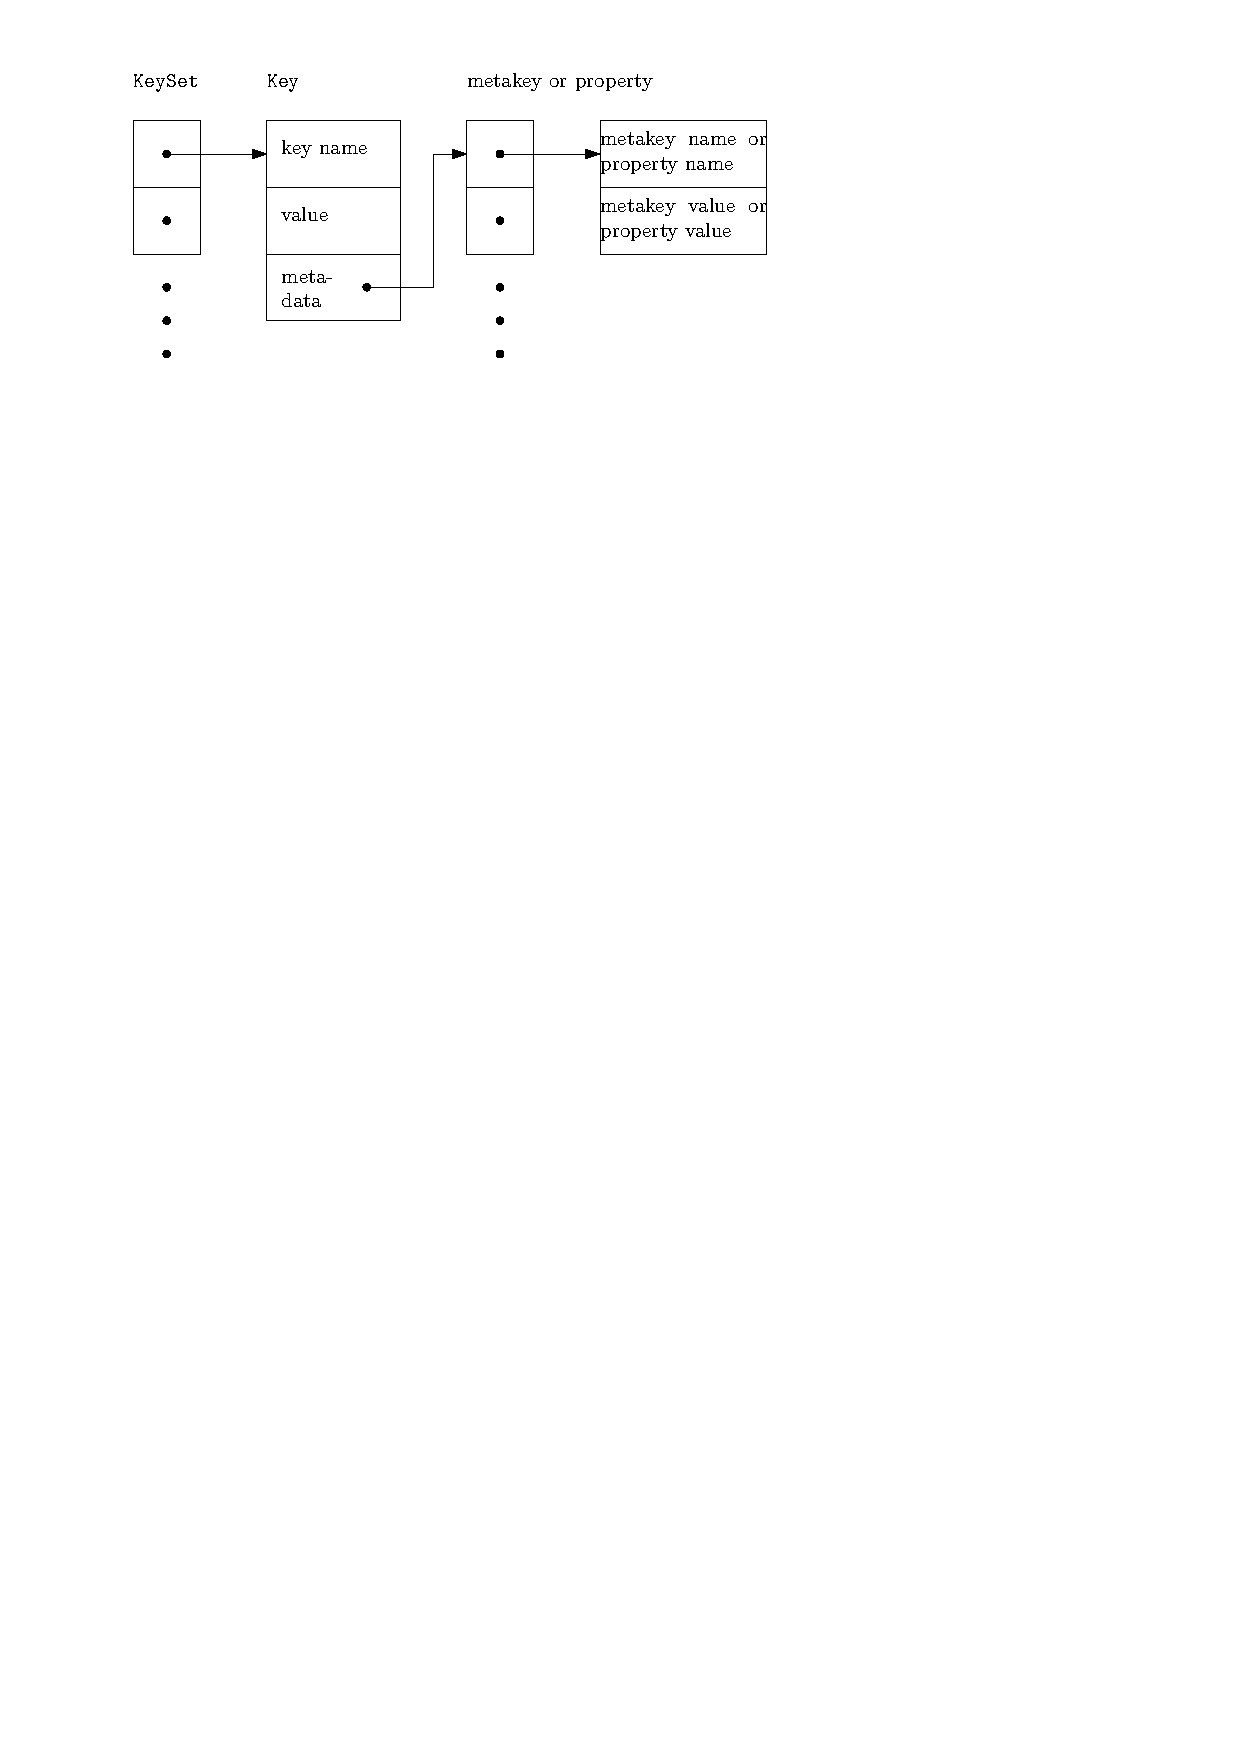
\includegraphics{keyset}
%\end{frame}
%
%\subsection{Assignments}
%
%\begin{frame}
%	\frametitle{Pull Requests}
%
%	\begin{task}
%	H0: public pull request
%	\end{task}
%
%	\begin{itemize}
%	\item build server and reviews take time
%	\item make sure to modify \texttt{doc/news/\_preparation\_next\_release.md} according to instructions
%	\item we use automatic formatter of code
%	\end{itemize}
%\end{frame}
%
%\begin{frame}
%	\frametitle{Install Elektra}
%
%	\begin{task}
%	Did you already install Elektra?
%	How did you do it?
%	\end{task}
%
%	For example via Docker image:
%	\begin{itemize}
%	\item Debian Buster
%	\item Alpine: \texttt{docker run -it elektra/elektra}
%	\end{itemize}
%\end{frame}
%
%\begin{assignment}
%	\begin{task}
%	Break.
%	\end{task}
%\end{assignment}
%
%\begin{frame}
%	\frametitle{First Steps with Elektra}
%
%	\begin{task}
%	How have your first steps been?
%	\end{task}
%\end{frame}
%
%\begin{frame}
%	\frametitle{Variant}
%
%	\begin{task}
%	T1: choose variant
%	\end{task}
%
%	\begin{itemize}
%	\item Change in T1: required -> require
%	\item Do you already have ideas for FLOSS?
%	\end{itemize}
%\end{frame}
%
%\begin{frame}
%	\frametitle{Homework}
%
%	\begin{task}
%	H1: Homework Topic?
%	\end{task}
%\end{frame}
%
%\begin{frame}
%	\frametitle{Feedback}
%	\hfill \includegraphics[width=2cm]{pics/feedback.png}
%	\vspace{-1cm}
%	\begin{itemize}
%		\item Please fill out in TUWEL
%		\item Reverse Classroom?
%		\item Materials?
%		\item Any suggestions for improvements?
%	\end{itemize}
%\end{frame}
%
%\subsection{L02: Configuration Specification Languages}
%
%\begin{frame}
%	\frametitle{Preview Next Week}
%
%	L02: Configuration Specification Languages
%
%	\begin{itemize}
%	\item to avoid misconfiguration
%	\item to allow systematic introspection
%	\item see TUWEL
%	\end{itemize}
%\end{frame}


%%%%%%%%%%%%%%%%%%%%%%%%%%%%%%%%%%%%%%%%%% 
\nocite{raab2017introducing}

\appendix

\begin{frame}[allowframebreaks]
	\bibliographystyle{plainnat}
	\bibliography{../shared/elektra.bib}
\end{frame}

\end{document}


